\section{Oferirea accesului unui utilizator}

Operatia de oferire a accesului unui nou utilizator presupune folosirea interfetei de administrare. Dupa setarea numeului noului utilizator si a parolei, noul cont este gata pentru folosit, iar pentru convenabilitate codul QR geenrat poate fi scanat cu aplicatia pentru a se autentifica automat

\begin{figure}[H]
\begin{center}
  \subfloat[Introducerea credentialelor noi]{\label{fig:useradda}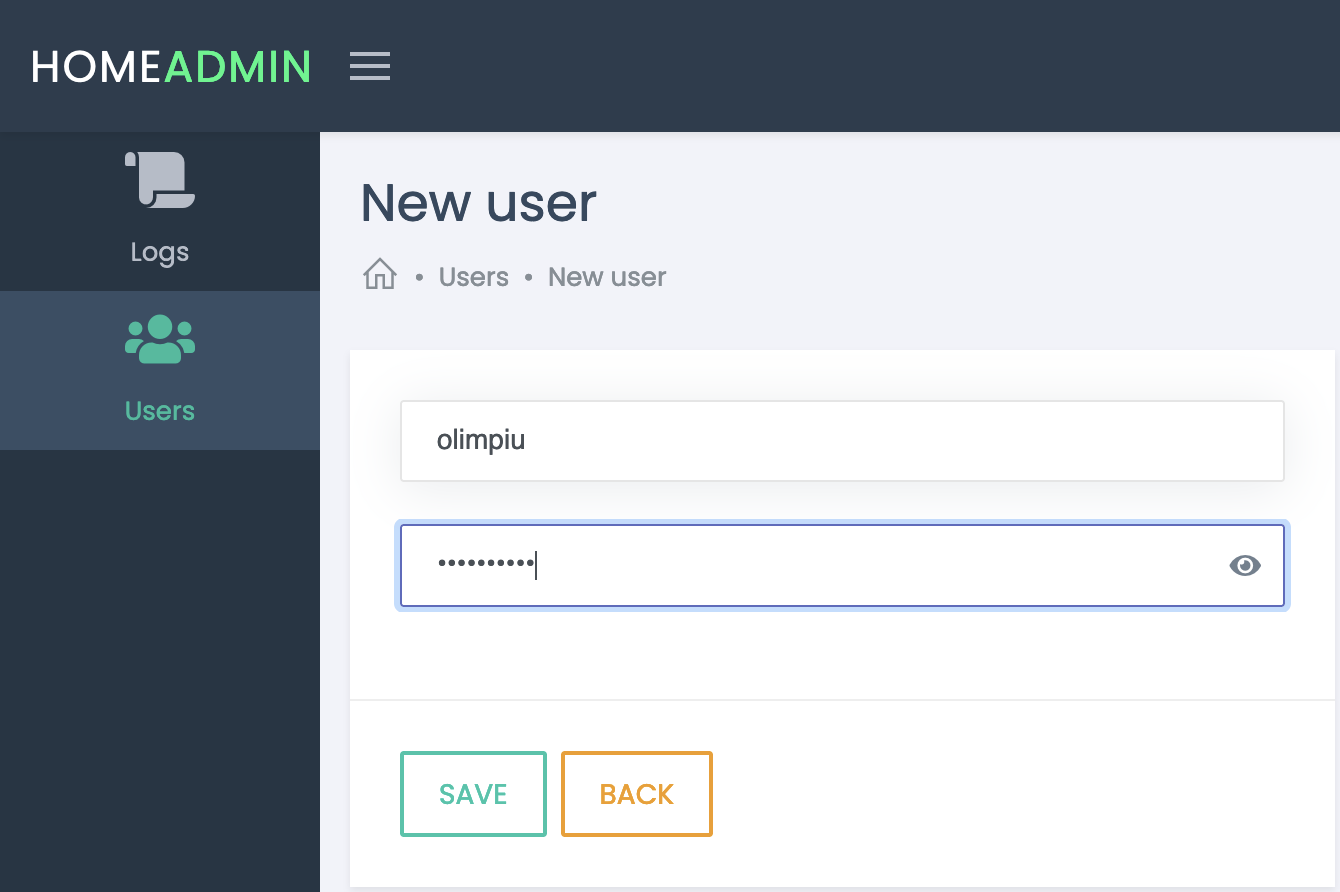
\includegraphics[width=\doublefigure]{05/06_admin_add_user.png}}
  \hfil
  \subfloat[Confirmarea adaugarii noului cont]{\label{fig:useraddb}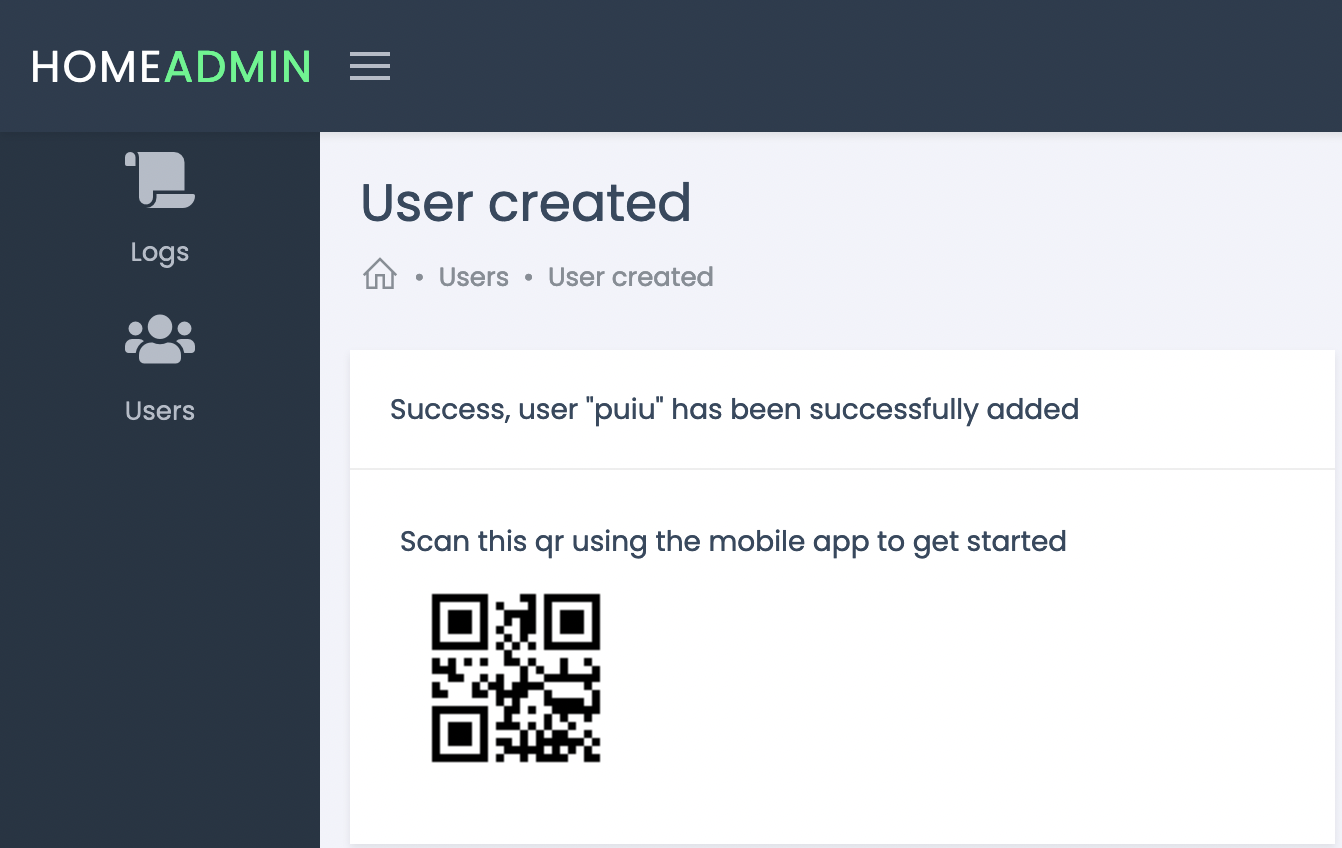
\includegraphics[width=\doublefigure]{05/07_admin_add_user_success.png}}
  \caption{Creare utilizator nou}
  \label{fig:useradd}
\end{center}
\end{figure}

Dupa descarcarea aplicatiei din Google Play Store, se va putea realiza autentificarea. Un alt avantaj al unui astfel de sistem este eliminarea nevoii cartelelor fizice, usor pierdut sau incurcat.

\begin{figure}[H]
\begin{center}
  \subfloat[Ecran autentificare aplicatie]{\label{fig:androidqra}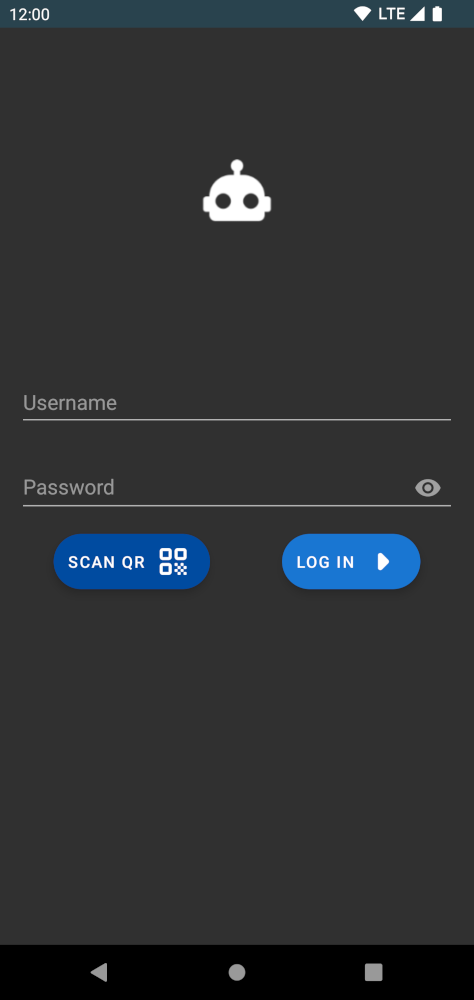
\includegraphics[width=\doublefigure]{05/08_android_log_in.png}}
  \hfil
  \subfloat[Scanarea codului QR]{\label{fig:androidqrb}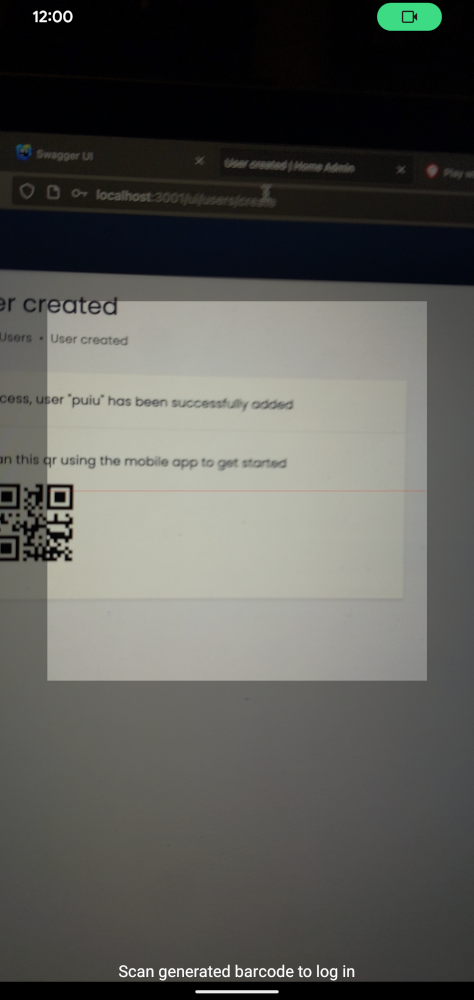
\includegraphics[width=\doublefigure]{05/09_android_qr.png}}
  \caption{Autentificare prin scanare cod QR}
  \label{fig:androidqr}
\end{center}
\end{figure}

\section{Raspuns automat}

Majoritatea vizitelor si apelurilor la interfon sunt previzibile, de exemplu venirea curierului sau a unui postas este anuntata printr-un interval aproximativ de timp. Deoarece utilizatorul duce o viata ocupata si stie ca urmeaza sa fie sunat, poate programa sistemul sa raspunda si sa deschida automat usa la urmatorul apel pentru o durata predefinita.

\begin{figure}[H]
\begin{center}
  \subfloat[Apasarea butonului albastru auto-answer va arata meniul pentru configurarea functionalitatii]{\label{fig:autoanswera}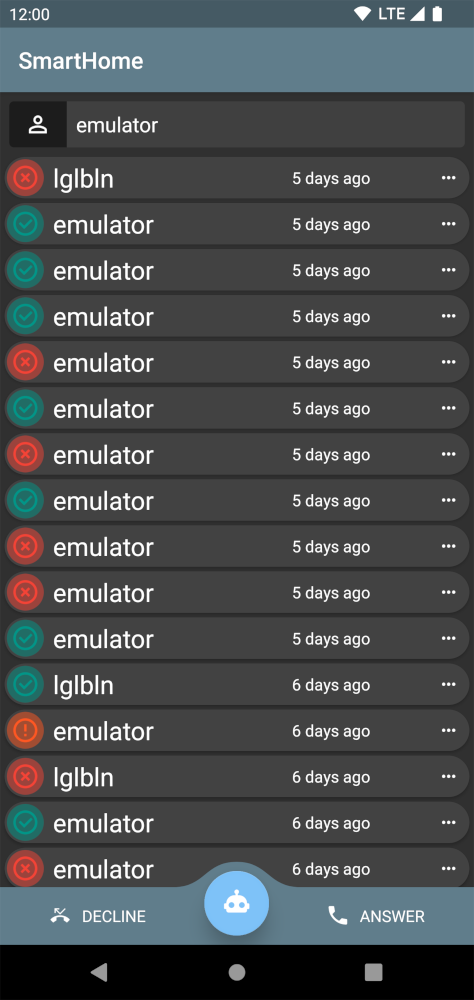
\includegraphics[width=\doublefigure]{05/01_android_autoanswer.png}}
  \hfil
  \subfloat[Alegerea unui interval pentru care functia va fi activa]{\label{fig:autoanswerb}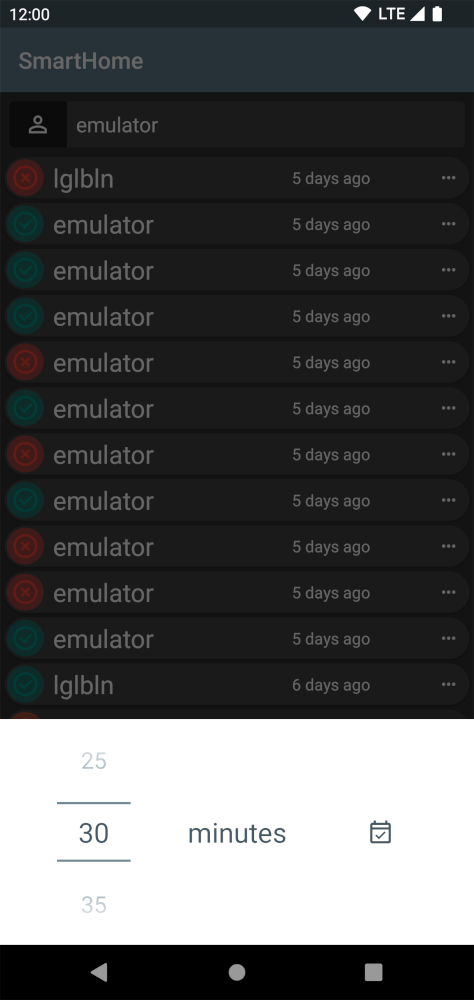
\includegraphics[width=\doublefigure]{05/02_android_auto_set.png}}
  \caption{Pasi pentru setare functie auto-answer}
  \label{fig:autoanswer}
\end{center}
\end{figure}

Se confirma activarea functiei prin colorarea butonului auto-answer in portocaliu. Intr-o maniera similiara, daca se doreste oprirea inainte de termen, se poate face acest lucru din meniul anterior.

\section{Raspuns de la distanta}

Prin conectarea la reteaua \acrshort{iot} sistemul este expus Internetului, acesta fiind avantajul solutiei, dar si unul din factori limitanti ai sai. Posibilitatea de deschidere de oriunde clientul are un dispzitiv conectat la Internet inseamna ca in lipsa cartelei standard \acrfull{rfid} se poate apela propriul apartament. Se va folosi aplicatia mobila pentru a se raspunde la propriul apel.

\begin{figure}[H]
\begin{center}
  \subfloat[In cazul in care aplicatia este pornita, utilizatorul este redirectat in IncomingActivity]{\label{fig:ringinga}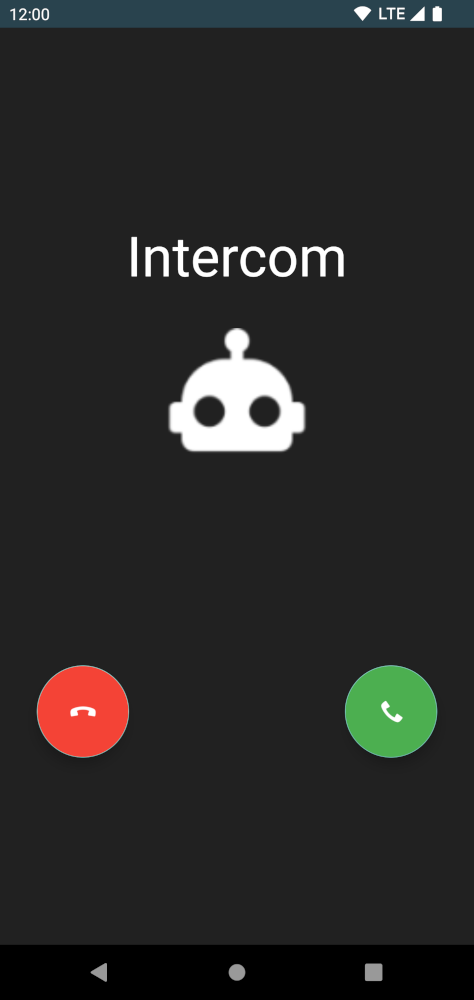
\includegraphics[width=\doublefigure]{05/04_android_app_ringing.png}}
  \hfil
  \subfloat[In cazul in care aplicatia nu este in foreground, se trimite o notificare de sistem cu doua actiuni]{\label{fig:ringingb}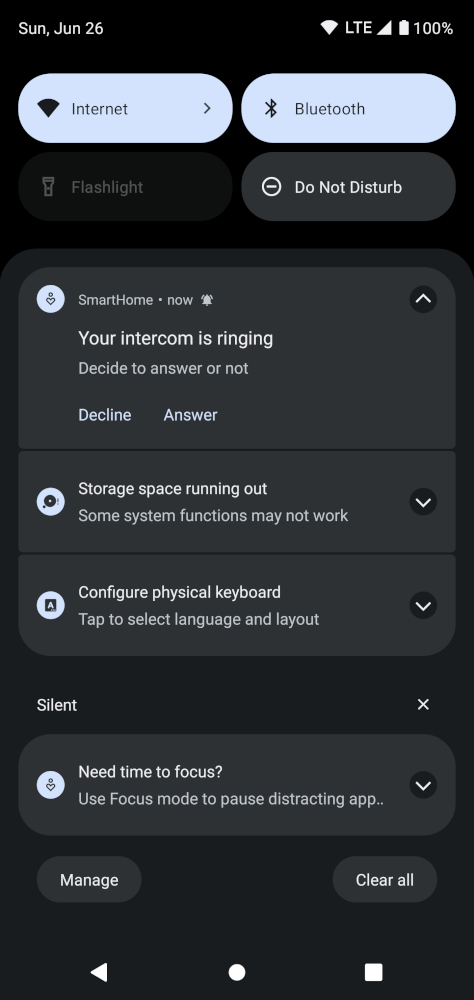
\includegraphics[width=\doublefigure]{05/05_android_notification_ringing.png}}
  \caption{Ecran apel}
  \label{fig:ringing}
\end{center}
\end{figure}

O alta varianta pentru mitigarea acestei probleme a fost folosirea unui tag \acrfull{nfc} care contine codat url-ul de acces impreuna cu un token care nu expira. Astfel prin scanarea lui cu un telefon ce dispune de anena \acrshort{nfc} se va realiza request-ul din browserul default al utilizatorului, rezultand in deschiderea interfonului.